\chapter{Implementation}

\section{Introduction} 

This chapter focuses on practical implementation with respect to the Domain Legitimacy Checker. The multi-viewed approach, along with programming in Python and the web framework in Flask, HTML, CSS, JavaScript, on the side of external APIs, assisted greatly in making a resilient framework for DNS abuse detection and transparency improvement. With those alternatives, I came up with this simple but effective way of not just finding legitimacy in domain names but also of showing plainly and clearly the various tactics with which bad actors are using in the adoption of confusable domains for phishing and malware distribution, along with other malicious activities to help me with my research. This endeavour embarked on a journey from ideation to execution, focusing on a user-friendly web interface that allows users to swiftly identify potentially malicious domains. 

\section{System Overview}

Domain Legitimacy Checker is such a robust web-based platform tasked with the identification and analysis of domain names that can be malicious. The user first initiates the requests of the domain names through the user interface. This request is processed by the Flask-based web server orchestrating the core operations of the system. Domain Analysis Engine is meant to perform an analysis on DNS abuse patterns exhibited by the submitted domain using heuristics and pattern matching algorithms. For a deep check, the system enqueues External APIs like VirusTotal over additional checks on the legitimacy. The results of such checking are kept in a Database as well, which gives out the history of known malicious domains. Finally, the Results Display component gives control of the results back to the user. Figure \ref{fig:figfig} provides an illustrative view of the architecture of design of the software system and information flow.


\begin{figure}[H]
\captionsetup{font= footnotesize}
    \centering
    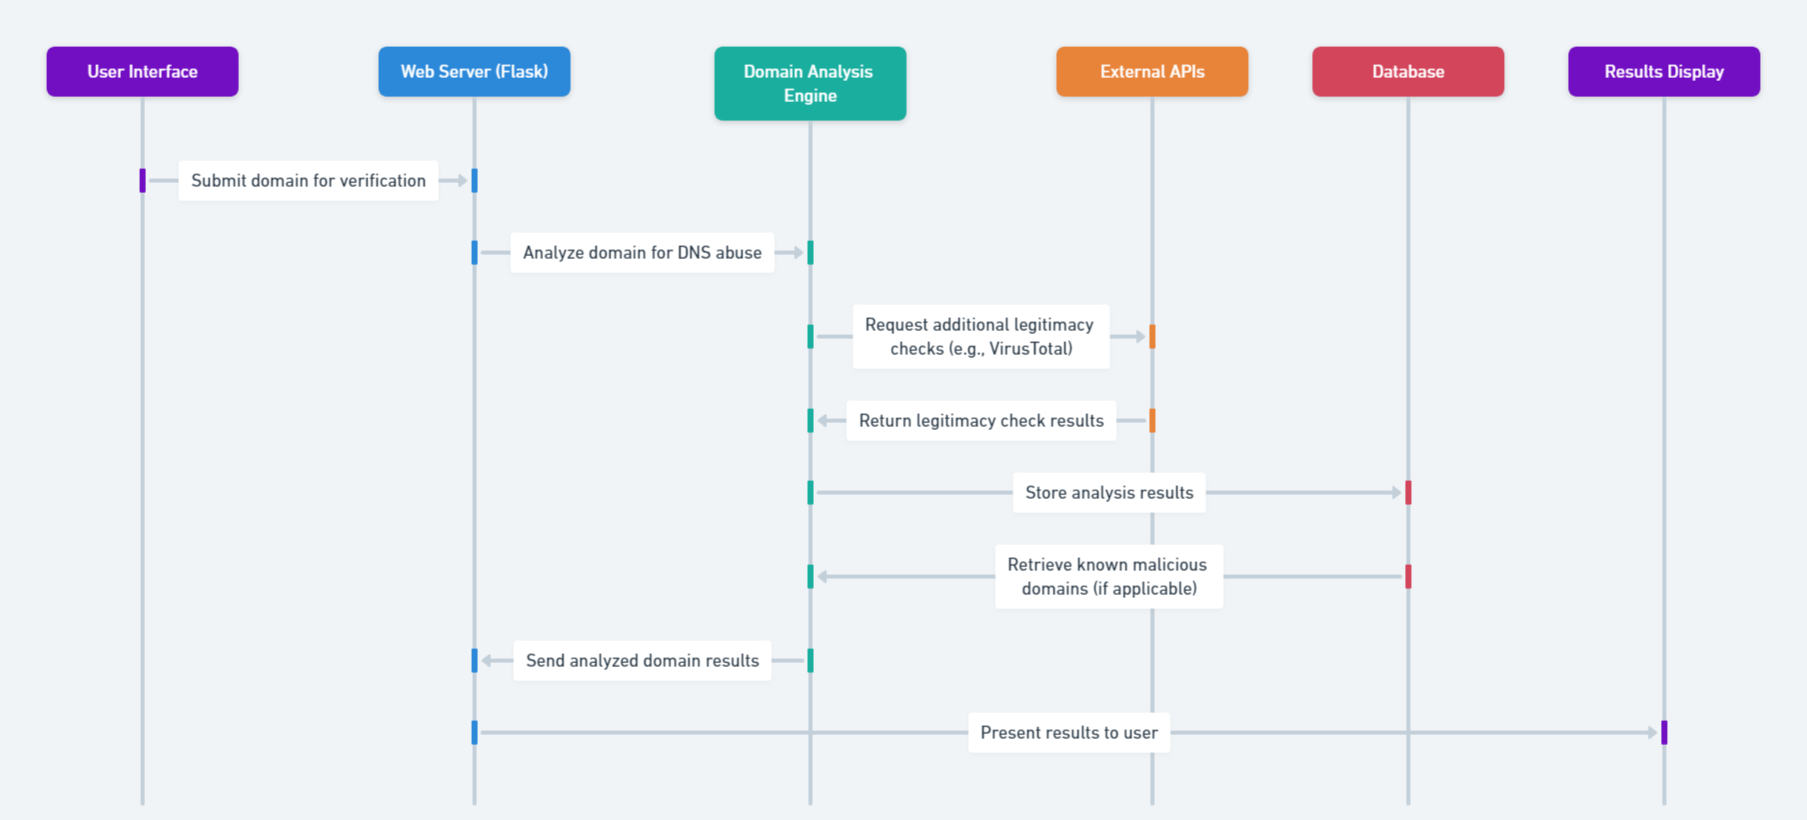
\includegraphics[width=1\linewidth]{project/DNS Abuse Transparency System.png}
    \caption{Domain Legitimacy Checker}
    \label{fig:figfig}
\end{figure}

\section{Integration} 
\subsection{Backend Implementation}

The server side :   Python on the Flask framework was used for implementing this side. The server works better with a solid web server in case you are time-pressed because the learning curve on Flask to make it implement is not that steep. The Flask application is set to work through a series of endpoints, each of which corresponds to a set of functionalities with respect to the system, among which is an endpoint for submitting domains to ascertain the results of their analysis. A request comes into the Flask server, and for any incoming given request, it simply calls the indicated function to handle the process relevant to the request: a process to parse the input data, to start domain checks, or to respond with the check results.

 API and library : The Domain Analysis Engine forms the main core within the backend, responsible for DNS abuse detection. This is realised by creating some of the changes that the submitted forms of domain names have so that possibly malicious or confusable counterparts are recognised with the assistance of pattern recognition algorithms. In addition, the development leverages libraries and packages such as "dnspython" and requests to conduct the queries to DNS and "request" APIs with respective libraries. This system communicates with external APIs such as "VirusTotal" in order to perform legitimacy checks, whereby the fact is made up for carrying out thorough analysis and reliable detection of malicious domains.

 \begin{figure}[H]
     \centering
     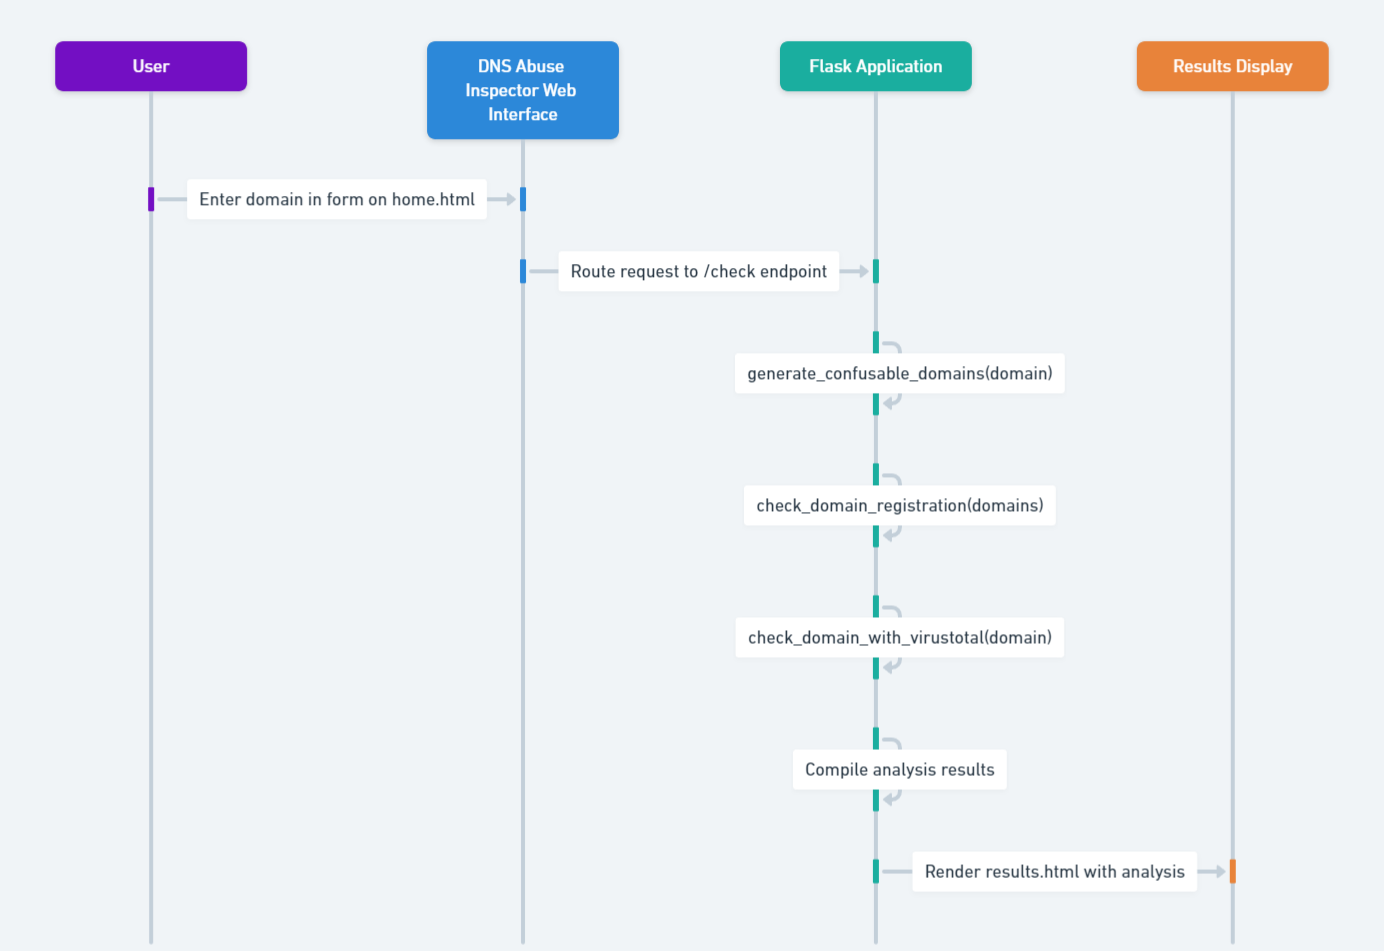
\includegraphics[width=1\linewidth]{project/Domain Legitimacy Check Workflow.png}
     \caption{Domain Legitimacy Checker System Interaction Workflow}
     \label{fig:figfigfig}
 \end{figure}

\subsection{Frontend Implementation}

Web Interface: HTML was used and then styled with CSS, and fine-tuned with Bootstrap, the user interface has responsiveness built in and is very user-friendly for use, regardless of the device that it is being used on. The interface is user-friendly, from submission of the initial domains easily, to displaying results, intending an automatically flowing process designed simple to the layman.


Interactive Elements: JavaScript is used to bring in interactivity to most of the pages, mostly through the main.js file, bringing the most important interactivity to the web app domain submission pages. These respects real-time, giving feedback even for the submission of domains, for instance changing the text of the submission button to "Analysing." and avoiding its swarming with submissions. These dynamic elements in the front-end make the process of domain analysis even more visually responsive, which increases users' engagements and trust in how the system processes.

\begin{figure}[H]
    \centering
    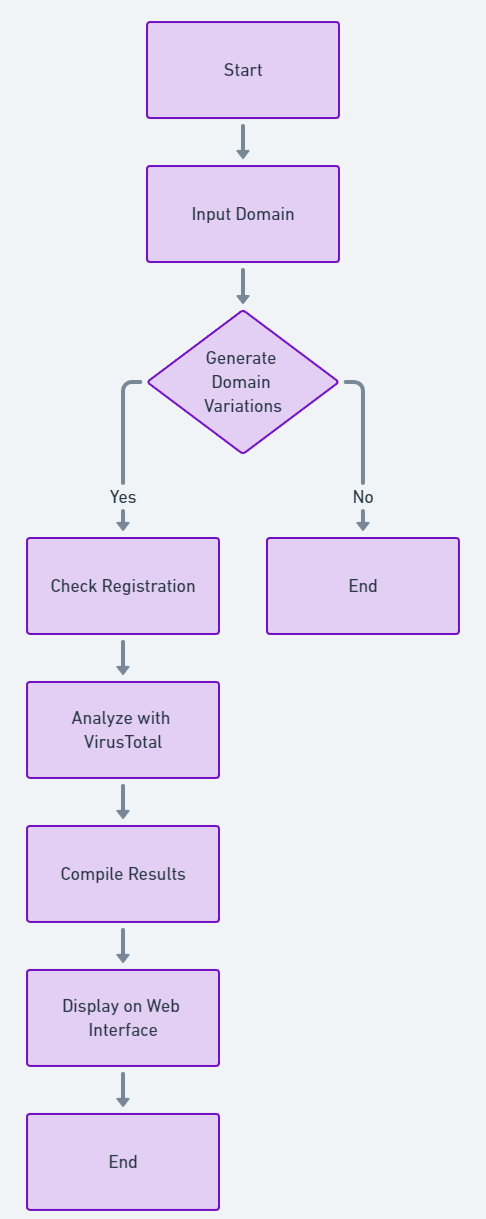
\includegraphics[width=0.6\linewidth]{project/DNS Abuse Inspector Operational Flowchart.png}
    \caption{Domain Legitimacy Checker}
    \label{fig:figfigfig}
\end{figure}
\newpage


\section{Tools and Technologies}

The Domain Legitimacy Checker was constructed using a carefully selected stack of tools, languages, and platforms. The primary language chosen was Python, valued for its readability, comprehensive standard library, and wide range of third-party modules that facilitate rapid development and integration with other systems. As a result, the decision was made to stick with Flask as an interactive back-end web framework, since in connection with its extremely light character, it's easily scalable and updatable in nature. Though designed very simple, it's versatile enough to really cover all major issues regarding painful threads of HTTP-requests processing.

For the frontend, HTML5 was the markup language of choice for structuring content on the web, while CSS3 was used for styling, ensuring a modern and engaging user interface. Bootstrap, a widely-used frontend framework, was integrated to expedite responsive design, allowing the interface to adapt to various device screens without extensive custom code. It is very important to ensure that a system runs smoothly by making the development of dynamic and interactive web pages using JavaScript. In the system, the scripting at the client side has used plain JavaScript so that it may maintain simplicity and hold onto any control over all the behaviours implicated.

The dnspython library provided the tools necessary for DNS queries, allowing the system to programmatically interact with DNS records, an essential feature for checking domain registration status. To conduct external checks for domain legitimacy, the requests library facilitated communication with external APIs, such as VirusTotal, renowned for its extensive database and reliable threat analysis. 

The VirusTotal API was used due to its comprehensive scanning capabilities, which leverage a multitude of antivirus engines and website scanners to assess the security of a domain. The scope of its scanning will come from thousands of antivirus engines and websites that will check if the domain is safe to browse or download. Equally important in the DNS Abuse System is the ability to establish the analysis of a wide spectrum of potentially abusive domains. VirusTotal searches for a record of if the supplied domain has ever been blacklisted before for hosting phishing sites, spreading malicious software, or, in general, being accessed for carrying out other suspicious actions. Such a dataset is to be found within the very repository of the API, thereby making available unmatched data and accuracy for threat detection, hence by and large enhancing the capability of this system in terms of protection against DNS related cyber threats.


Each tool and technology were chosen not only for its individual merits, but also for how well it integrated with the others, ensuring a cohesive and efficient system aligned with the project's objectives of DNS abuse detection and transparency.


\section{Challenges and Solutions}

During the development of the Domain Legitimacy Checker, I faced several challenges, each requiring a tailored solution to ensure the project's success.

Challenge 1: API Rate Limiting
The frequent use of the VirusTotal API presented a challenge due to its rate-limiting constraints. Exceeding the allotted number of requests would lead to temporary blocking of our service.

Solution: Implementing a queuing system with a delay mechanism to spread the requests over time, adhering to the API's rate limits. Additionally, we cached the results of previous queries to minimise repeat requests for the same domains.

Challenge 2: Real-time Feedback for Users, therefore, very important to give very instant feedback in the process of the domain analysis but was otherwise very hard to prove because of the asynchronous behaviour, in principle for network operations.

Solution: Using asynchronous JavaScript to send information to the servers and receive results from them without refreshing the web page. The user also receives a form of visual indication in the form of a bar on the point of progress as the analysis unfolds in real time.

Challenge 3: Handling Malicious Domain Variations
Identification and generation of a full set of confusing domain variations represented a key computational challenge.
Solution: Utilising a combination of common substitution algorithms and a heuristic approach that prioritised variations based on their likelihood of being used in phishing attacks. That way, it helped us match the balance of well-performed search against the practical need for it and against timely results.

Challenge 4: Data Storage and Retrieval Efficiency
Storing analysis results for quick retrieval while managing database performance was a concern, especially with the growth of the dataset.
Solution: Selecting a suitable relational database management system with efficient search capability in terms of indexing and structured schema that would help provide faster lookup. Regular maintenance routines were established to optimise database performance.

Challenge 5: System Scalability
As the system's user base grows, so does the load on our servers, which initially led to concerns about scalability.
Solution: The system was architected with scalability in mind, using Flask's built-in capabilities to handle an increasing number of simultaneous user requests. 
By addressing these challenges with careful planning and adaptive solutions, we enhanced the system's reliability, performance, and user satisfaction.

\section{Testing and Validation}

Domain Legitimacy Checker follows rigorous measures in testing the system, which assures both dependability and accuracy. In the implementation, back-end logic had the number of things implemented with unit tests; we have used the Python unittest framework. We used mock objects for simulating the acts of the external APIs.

Both manual and automated testing were conducted in front-end technologies. Automated UI testings, such as with Selenium, were relied upon to ensure all interactive elements are operable. The interface has been tested both automatically and manually, with the help of loading a page on a few browsers and mobile devices to guarantee the interface is responsive and behaves alike.

I have done practice methodologies of test-driven development (TDD) within overall projects to simulate a lot of real-time scenarios. It will thus ensure the detection of the problem automatically in the early stage, which is necessary for further appropriate rectification. We also set up Continuous Integration (CI) pipelines that would fire every time a new code commit passes to run tests, ensuring newly made changes do not break existing functionalities automatically.

This was done by the system validation against known patterns of DNS abuse, and explanatory notes on the results are attached. Regular peer reviews were also held at regular intervals for the same purpose of reassessment of performance and reliability of the system.


\section{Conclusion}

The implementation of the DNS Abuse Transparency Reporting system reflects a significant stride towards addressing the complexities of domain name security. The chapter presented how integration of these different technologies finally translated into implementation of the platform on the ground for DNS abuse detection, which had reliable results. Key learnings included at what point the right tools should be chosen when it came to scaling and how testings done in an iterative way make the different functionalities stronger. Future enhancements could focus on incorporating artificial intelligence to predict emerging DNS abuse tactics and expanding the database for malicious domain variations. Continuous improvement in response to evolving cyber threats will bolster the system's capability to safeguard users in the digital landscape.
